%!TEX root = ../thesis.tex
%*******************************************************************************
%*********************************** First Chapter *****************************
%*******************************************************************************
\chapter{Markov Processes}~\label{chap:markov_processes}

\ifpdf%
    \graphicspath{{Chapter1/Figs/Raster/}{Chapter1/Figs/PDF/}{Chapter1/Figs/}}
\else
    \graphicspath{{Chapter1/Figs/Vector/}{Chapter1/Figs/}}
\fi

\tikzstyle{state}=[shape=circle, draw=blue!50,fill=blue!20]
\tikzstyle{observation}=[shape=rectangle, draw=orange!50,fill=orange!20]
\tikzstyle{lightedge}=[<-, dotted]
\tikzstyle{mainstate}=[state, thick]
\tikzstyle{mainedge}=[<-, thick]

As described in \citep{Ross2014}, a Markov chain is a stochastic process describing a sequence of possible events where the probability of each event depends solely on the state attained in the previous event. This is termed as the 'Markov Property', which encapsulates the memorylessness of the process — the future is independent of the past given the present.

Markov chains provide a robust framework for modeling the probabilistic nature of cryptocurrency markets. The rapid fluctuation of cryptocurrency prices, driven by a myriad of factors such as market sentiment, technological advancements, regulatory news, and macroeconomic trends, may be represented effectively using Markov chains.~\citep{Zhang2023}

In this chapter, we start by laying down the fundamental theoretical foundations of Markov chains. This includes an explanation of key concepts such as state spaces, transition probabilities, and the difference between discrete and continuous time Markov chains. Understanding these basic building blocks is pivotal in leveraging Markov chains for cryptocurrency market analysis and trading.

Next, we focus on specific properties of Markov chains like irreducibility, periodicity, and stationarity, which play critical roles in determining the long-term behavior of the chain.

%********************************** %First Section  **************************************
\section{Discrete-time Markov Chains}~\label{sec:dtmc}

Since we know that Markov Chain is a stochastic process, we ought to define what a stochastic process is, in itself, first. 

Let $\Omega \neq \emptyset$ and $\mathcal{F} \subseteq 2^{\Omega}$ be a $\sigma$-algebra on $\Omega$, and $\mathbb{P}$ a measure with $\mathbb{P}(\Omega) = 1$, i.e. $\mathbb{P}$ is a \textit{probability measure}. According to \citep{Dostal}, the triplet $(\Omega, \mathcal{F}, \mathbb{P})$ is, in this case, called a \textit{discrete probability space}. Where $\Omega$ denotes a sure event, and it holds that $\forall \omega \in \Omega$ is called an \textit{elementary event}. Furthermore, $\forall A \in \mathcal{F}$ is a random event  so that $\mathbb{P}(A)$ denotes a probability of that event. 

Let $I$ be a countable set and $\mathbb{S}$ a $\sigma$-algebra on $I$. Each $i \in I$ is called a \textit{state} and $(I,\mathbb{S})$ a \textit{state-space}.
Therefore, we have two measurable topological spaces $(\Omega,\mathcal{F})$ and $(I,\mathbb{S})$ and a random variable $X: \Omega \rightarrow I$ assuming that X is measurable function. Thus, we call $(I,\mathbb{S})$ a state space and $(\Omega, \mathcal{F})$ an underlying space. Therefore, we may set:

\begin{equation}
\mu_X(i) = \mathbb{P}(X=i)=\mathbb{P}(\{\omega: X(\omega)=i\})
\end{equation}

Since we are allowing only for the discrete realizations of the random variable X, given previous assumptions and that $\sum\limits_{i \in I} \mu_X(i)=1$, $\mu_X$ is a \textit{probability mass function}.~\citep{Norris2012}

Let us now assume that we have a sequence of random variables $\{X_t : t \in T\}$ where $T$ is a countable set of time steps.
 We say that $\{X_t : t \in T\}$ is a \textit{stochastic process} and if it also holds that $T \in \mathbb{N}_0$ then \textit{discrete-time stochastic process}.
 In the context of Markov Chains we call measurable space $I$ as a \textit{state space} and $X_t$ as a \textit{state} at time $t$ respectively.
 Given the initial setup, we may define a \textit{discrete-time Markov Chain (DTMC)} as a stochastic process $\{X_t : t \in T\}$ with a state space $I$ and a distribution $\mu_X$ such that for all $t \in T$ and $i_0,i_1,\ldots,i_{t+1} \in I$ it holds that:

\begin{equation} \label{eq:DTMC}
\mathbb{P}(X_{t+1}=i_{t+1}|X_t=i_t,\ldots,X_0=i_0) = \mathbb{P}(X_{t+1}=i_{t+1}|X_t=i_t)
\end{equation}

according to \citep{Praskova2012}. In other words, the probability of observing a state $i_{t+1}$ at time $t+1$ given the sequence of states $i_0,i_1,\ldots,i_{t}$ is equal to the probability of observing a state $i_{t+1}$ at time $t+1$ given only the last observed state $i_t$.
This fundamental relationship is called \textit{Markov property}, and it is a consequence of the \textit{memoryless property} of Markov Chains.~\citep{Haggstrom2002}

Conditional property of Markov Chains may be equivalently expressed using a future state $j \in I$ and a current state $i \in I$ as:

\begin{equation}
    \mathbb{P}(X_{t+1}=j|X_t=i) = p_{i,j}(t,t+1)
\end{equation}

where $p_{i,j}(t,t+1)$ is a \textit{transition probability} from state $i$ to state $j$ at time $t$ and $t+1$ respectively. Sometimes we refer to these transitions as \textit{one-step transitions} since they are only dependent on the previous state.
As an extension of the Markov property we may also define a \textit{k-step transition} as a probability of observing a state $j$ at time $t+k$ given the state $i$ at time $t$ as \citep{Tolver2016}:

\begin{equation}
    \mathbb{P}(X_{t+k}=j|X_t=i) = p_{i,j}(t,t+k)
\end{equation}

One important distinction by \citep{Weinan2019} is that if the transition probabilities $p_{j,i}(t,t+k)$ do not depend on time $t$ then the Markov Chain is called \textit{homogeneous} otherwise these probabilities vary over time, therefore \textit{heterogeneous} Markov Chain\footnote{In some sources the homogeneity with respect to time is emphasized s.t.\ the term is time-homogeneous or time-heterogenuous Markov Chain.}.

Considering only first order homogeneous Markov Chain we may define a \textit{transition matrix} 
$A = (p_{i,j} : i,j \in I)$ as a matrix of transition probabilities between each state $i,j \in I$ such that:

\begin{equation} \label{eq:1.5}
    p_{i,j} \geq 0 \quad i,j \in I; \quad \sum\limits_{j \in I} ^{}p_{i,j} = 1, \quad \forall i \in I
\end{equation}

Rectangular matrix $\textbf{A}$ that satisfies property given by Equation~\ref{eq:1.5} is called \textit{stochastic matrix}.~\citep{Gagniuc2017}
Furthermore, we ought to define a probability distribution $\textbf{p} =\{p_i, i \in I\} $ as a vector of probabilities of observing each state at time $t=0$ such that:

\begin{equation}
p_i = \mathbb{P}(X_0=i), \quad i \in I
\end{equation}

and 

\begin{equation}
p_i \geq 0 \quad i \in I; \quad \sum\limits_{i \in I} p_i = 1
\end{equation}

\noindent which is also called the \textit{initial distribution} of Markov Chain.

According to~\citep{Praskova2012}, once we have transition matrix $A$ and initial distribution $\textbf{p}$ that satisfy constraints given by Equation (1.5) and (1.7) respectively,
then $\{X_t,t \in \mathbb{N}_0\}$ is a discrete-time homogeneous Markov Chain with transition matrix $A$ and initial distribution $\textbf{p}$ 
if and only if all finite dimensional distributions of $\{X_t\}$ are consistent with the following equation:

\begin{equation} \label{eq:kolmogorov}
    \mathbb{P}(X_{0}=i_0,X_{1}=i_1,\ldots,X_{t}=i_t) = p_{i_0} a_{i_0,i_1} \ldots a_{i_{t-1},i_t}
\end{equation}

where $i_0,i_1,\ldots,i_t \in I$. If we abstract from the initial distribution $\textbf{p}$, such equation is called \textit{Chapman-Kolmogorov equation} as in~\citep{Yin2004}.
Equation~\ref{eq:kolmogorov} also holds for heterogenuous Markov Chains where the transition probabilities $p_{i,j}$ are time dependent:

\begin{equation}
    \mathbb{P}(X_{0}=i_0,X_{1}=i_1,\ldots,X_{t}=i_t) = p_{i_0}(0) p_{i_0,i_1}(0,1) \ldots p_{i_{t-1},i_t}(t-1,t)
\end{equation}

Another substantial property of homogeneous Markov Chains is that their n-th order transition probabilities can be expressed as a product of their first order transition probabilities:

\begin{equation}
    \mathbb{P}(X_{m+n} = j|X_{m} = i) = a_{i,j}^{(n)}, \quad i,j \in I
\end{equation}

where generally $a_{i,j}^{(m+n)} = \sum\limits_{k \in I} a_{i,k}^{(m)} a_{k,j}^{(n)}$ is referred to as \textit{Chapman-Kolmogorov equality} and holds for $m,n \in \mathbb{N}_0$ and $\mathbb{P}(X_m=i) \geq 0$.~\citep{Praskova2012}

To simply illustrate the idea behind discrete-time Markov Chains let us assume a situation where the future market movements transition between a countable number of states $I =$ \{upward, side, downward\} 
and there is an arbitrary transition matrix \textbf{A} and initial distribution \textbf{p}:

\begin{equation}
    \textbf{A} =
\begin{pmatrix}
0.1 & 0.4 & 0.5 \\
0.25 & 0.3 & 0.45 \\
0.33 & 0.33 & 0.33 
\end{pmatrix} 
, \quad \textbf{p} = 
\begin{pmatrix}
    0.2 & 0.3 & 0.5 \\
\end{pmatrix}
\end{equation}

using a maximum likelihood estimator of transition matrix according to \citep{Gagniuc2017} with $T$ being the length of the sequence of states:

\begin{equation}
    \hat{a}_{i,j} = \frac{\sum\limits_{k=1}^{T-1} \mathbbm{1}_{\{X_k=i,X_{k+1}=j\}}}{\sum\limits_{k=1}^{T-1} \mathbbm{1}_{\{X_k=i\}}}
\end{equation}

Each row represents full set of transition probabilities between states, also visible from $\sum\limits_{j \in I} a_{i,j} = 1 $, i.e.\ each row of matrix $\textbf{A}$ represents a conditional probability distribution given $i \in I$. 
Such a relationship can be represented as a diagram indexing each state by U, S and D respectively as follows:

\begin{figure}[htbp]
\begin{center}
\begin{tikzpicture}[->, >=stealth', auto, semithick, node distance=3cm]
\tikzstyle{every state}=[fill=white,draw=black,thick,text=black,scale=1]
\node[state]    (U)               {$U$};
\node[state]    (S)[right of=U]   {$S$};
\node[state]    (D)[right of=S]   {$D$};
\path
(U) edge[loop left]             node{$0.1$}   (U)
    edge[bend left,above]       node{$0.4$}   (S)
    edge[bend right=55,below]   node{$0.5$}   (D)
(S) edge[bend left,above]       node{$0.45$}  (D)
    edge[loop below]            node{$0.3$}   (S)
    edge[bend left, below]      node{$0.25$}  (U)
(D) edge[bend right=55,above]   node{$0.33$}  (U)
    edge[loop right]            node{$0.33$}  (D)
    edge[bend left, below]      node{$0.33$}  (S);
\end{tikzpicture}
\caption[Visual representation of discrere-time Markov Chain]{Transition diagram of the discrete-time Markov Chain given transition matrix \textbf{A}.}
\end{center}
\end{figure}

This may be easily interpreted for each given state. For example if we assume that the market moved upwards on the last trading day there is a 0.1 chance that the market will move in positive direction today, in other words the conditional probability of observing the state U today given the state U yesterday is 0.1. 
On the hand if we suppose that today the market actually transitioned to the state S with probability 0.4 there is now a probability of 0.45 to transition to state D since the future transition is only conditioned by its previous state. 

Suppose now that we have observed a given sequence of states for the last week as $\{U,S,D,D,U\}$, and we would like to know the sequence joint probability given the transition matrix $\textbf{A}$ and initial distribution $\textbf{p}$:

\begin{align}
\mathbb{P}(X_{t_0} = x_0,\ldots,X_{T} = x_T|\textbf{A},\textbf{p}) &= \mathbb{P}(X_0 = x_0) \prod_{k=1}^{T} \mathbb{P}(X_k=x_k|X_{k-1}=x_{k-1})\\
&= p_{x_0} a_{x_0,x_1}  a_{x_1,x_2}  a_{x_2,x_3} a_{x_3,x_4} \notag\\
&= 0.2 \times 0.4 \times 0.45 \times 0.33 \times 0.33 \notag\\
&= 0.002376 \notag
\end{align}

Where the probability of observing state $x_0$ is determined by our initial distribution $\textbf{p}$ since we have no prior knowledge about what exactly happened before $t=0$. 
Also, the joint probability of large sequences obviously results in very small numbers, so it is more convenient to work with logarithms of probabilities.

On the other hand, we might consider a situation in which we have observed such a sequence of events, 
and we need to determine the next state given entire sequence. As in the last example, 
we have our transition matrix $\textbf{A}$ and a sequence of events $\{U,S,D,D,U\}$ observed until $T$. 

We know that last observed state was $U$ which directs us straight to the first row of $\textbf{A}$ since from the properties of Markov Chains we know that the next state will depend solely on the present state, 
so we can abstract from the given sequence of past states and focus only on $X_{T}$. Finally, we may conclude that the most likely future state at time $T+1$ is $D$ with the probability of 0.5. Formally we may write:

\begin{equation}
 x_{T+1}^* = \underset{j \in I}{\arg\max} \mathbb{P}(X_{T+1}=j|X_{T}=x_T) \\
\end{equation} 

\subsection{Classification of states}

Markov Chains may be classified into several categories based on their properties. 
Firstly, \citep{Praskova2012} and others, distinguish between \textit{transient} and \textit{recurrent} states and as a convenient notation we will introduce so-called \textit{return time} $\tau_j$ 
as a random variable that denotes the time of k-th return to state $j \in I$:

\begin{equation}
\tau_j(k+1) = \inf \{T \geq \tau_j(k) : X_T =j\}, \quad k \in \mathbb{N}_0
\end{equation}

\noindent and if $\tau_j(k) \leq \infty$ and we assume that $\inf\{\emptyset\} = \infty$ and $\tau_j(0) = 0$.

This random variable also satisfies properties of \textit{recurrence time}. 
Any random variable $\tau:\Omega \to \mathbb{N}_0 \cup \{ \infty \}$ for which outcomes $[\tau = T]$ belong to 
$\sigma$-algebra $\mathcal{F}_T = \sigma(X_0,\ldots,X_T)$ generated by sequence of random variables $\{X_0,X_1, \ldots , X_T\}$ is called a \textit{recurrence time}.

Thus, \citep{Bremaud1999} and \citep{Tolver2016}, state that $j \in I$ is \textit{transient} if there is a non-zero probability that the process will never return to state $j$ once it has left it, i.e.:

\begin{equation}
    \mathbb{P}(\tau_j(1) < \infty|X_0=j) < 1, \quad \sum\limits_{n=0}^{\infty} a_{j,j}^{(n)} < \infty
\end{equation}

for some $k \in \mathbb{N}_0$. On the other hand, a state $j \in I$ is called \textit{recurrent} if it is not transient, i.e.:

\begin{equation}
    \mathbb{P}(\tau_j(1) < \infty|X_0=j) = 1, \quad \sum\limits_{n=0}^{\infty} a_{j,j}^{(n)} = \infty
\end{equation}

We can further distinguish between \textit{positive recurrent} if the expected return time is finite $\mathbb{E}[\tau_j(1)|X_0=j] < \infty$ and \textit{null recurrent} if the expected return time is infinite $\mathbb{E}[\tau_j(1)|X_0=j] = \infty$.

Let us make one more distinction regarding a Markov chain states as \citep{Gebali2008}. The greatest common divisor of the number of times a state can return to itself is the period. If the period is larger than 1, the state is called \textit{periodic} and 
on the contrary, if there is no such integer and the state can be revisited at any time, then the state is called \textit{aperiodic}.
If all states in a Markov chain are aperiodic, the Markov chain itself is said to be aperiodic as well. Aperiodicity is a desirable property for a Markov chain because it ensures that the chain does not get trapped in oscillating sequences of states. 
To clarify, a periodicity does not mean that each state must be reachable from every other state in just one step. It's a more subtle concept, meaning that the greatest common divisor of the lengths of all cycles in the chain must be 1, so that any state can be reached from any other state in a variable number of steps.

Previous properties of states lead us to define \textit{ergodic} state for which it holds that it needs to be positive recurrent and aperiodic. Such trait is substantial since it implies that the state will be visited infinitely often and the expected time between visits is finite.
Same logic applies that if all states of a Markov chain are ergodic, then the chain itself is ergodic and thus irreducible, i.e.\ all states communicate with each other.

\subsection{Stationary distribution}

A pivotal concept linked to Markov Chains is that of the stationary distribution, a distinct probability 
distribution that remains invariant under the transition dynamics of the chain. 
If we denote $\pi = \{\pi_j,j \in I\}$ as a probability distribution, and it satisfies following equality by \citep{Bremaud1999}:

\begin{equation} \label{eq:stationary}
    \pi_j = \sum_{i \in I} \pi_i a_{i,j}, \quad j \in I
\end{equation}

then $\pi$ is called a \textit{stationary distribution} of Markov Chain. That also implies that if the initial distribution of homogeneous Markov Chain is stationary in the sense of Equation~\ref{eq:stationary}
then Markov Chain is called strictly stationary stochastic process since the joint distribution of any finite number of random variables is invariant under the transition dynamics of the chain.
More specifically, for any $t,k \in \mathbb{N}_0$ and $i_0,i_1,\ldots,i_t \in I$ it holds that:

\begin{equation}
    \mathbb{P}(X_0=i_0,X_1=i_1,\ldots,X_t=i_t) = \mathbb{P}(X_k=i_0,X_{k+1}=i_1,\ldots,X_{k+t}=i_t)
\end{equation}

and also for $\pi_j$ called initial stationary probabilities:

\begin{equation} \label{eq:init_stationary}
    p_j(t) = \mathbb{P}(X_t = j) = \pi_j, \quad j \in I
\end{equation}

It's important to stress that the existence and uniqueness of a stationary distribution 
is not guaranteed for all Markov Chains, but under specific conditions a unique stationary 
distribution does exist and any initial distribution converges to this stationary distribution \citep{Praskova2012} as time progresses.
If all states of the chain are transient or null recurrent, then no stationary distribution exists. On the other hand if the chain is
positive recurrent, then a stationary distribution exists and is unique.

Important property of stationary distribution is that if we have an irreducible and aperiodic Markov Chain, 
its transition matrix $\textbf{A}$ converges to limiting matrix $\pi_{i,j}$ according to \citep{Haggstrom2002} as follows:

\begin{equation}
    \lim_{n \to \infty} a_{i,j}^{(n)} = \pi_{i,j}, \quad i,j \in I
\end{equation}

since the transition matrix is irreducible, each row entry of limiting matrix $\pi_{ij}$ is equal to the stationary distribution $\pi_j$. This is called \textit{Markov Chain convergence theorem}, and it implies that if we run 
Markov Chain for sufficiently long time, the distribution at time n approaches the stationary distribution $\pi$, i.e.\ approaches equilibrium as $n \to \infty$.
 
The fundamental significance of the stationary distribution arises from its ability to dictate the long-term, 
steady-state behavior of the chain. Furthermore, the stationary distribution plays an essential role in the 
calculation of expected return times, the analysis of limiting probabilities, and \citep{Navarro2011} states that it forms the backbone of
algorithms such as the Metropolis-Hastings algorithm widely used in Markov Chain Monte Carlo (MCMC) simulations which are described
in more detail in Section~\ref{sec:mcmc}.

\subsection{Cryptocurrency market movements I.}

The probabilities in previously introduced transition matrix $\textbf{A}$ were imaginary and served only as a mere example of the main properties of discrete-time Markov Chains. 
For now consider a dataset of BTC-USDT daily close prices from public cryptocurrency exchange Binance website from 23rd August 2020 to 15th May 2023. 
Firstly, we ought to make several assumptions about the data in order to satisfy properties of Markov Chains, namely define finite state space, transition period and memoryless process. 

\begin{itemize}
\item [1)] \textbf{Transition period}: We will define a transition period as a day, i.e.\ the transition probabilities will be calculated for each day.
\item [2)] \textbf{State space}: We will define a state space as a set of 3 states \{upward, side, downward\} which will be determined by the percentage change of the close price of the current day with respect to the previous day as follows:
    \begin{itemize}
    \item [a)] \textbf{Upward}: If the percentage change of the close price of the current day with respect to the previous day is greater than 0.5\%.
    \item [b)] \textbf{Side}: If the percentage change of the close price of the current day with respect to the previous day is between -0.5\% and 0.5\%.
    \item [c)] \textbf{Downward}: If the percentage change of the close price of the current day with respect to the previous day is less than -0.5\%.
    \end{itemize}
\item [3)] \textbf{Memoryless process}: We will assume that the future state of the market only depends on the current state, i.e.\ the transition probabilities are independent of time.
\end{itemize}

Given these assumptions we first examine BTC-USDT close price time series data in~\ref{fig:BTC-USD} and the distribution of the percentage change of the close price of the current day with respect to the previous day as shown in Figure~\ref{fig:BTC-USD-distribution}.

\begin{figure}[htbp]
    \begin{center}
        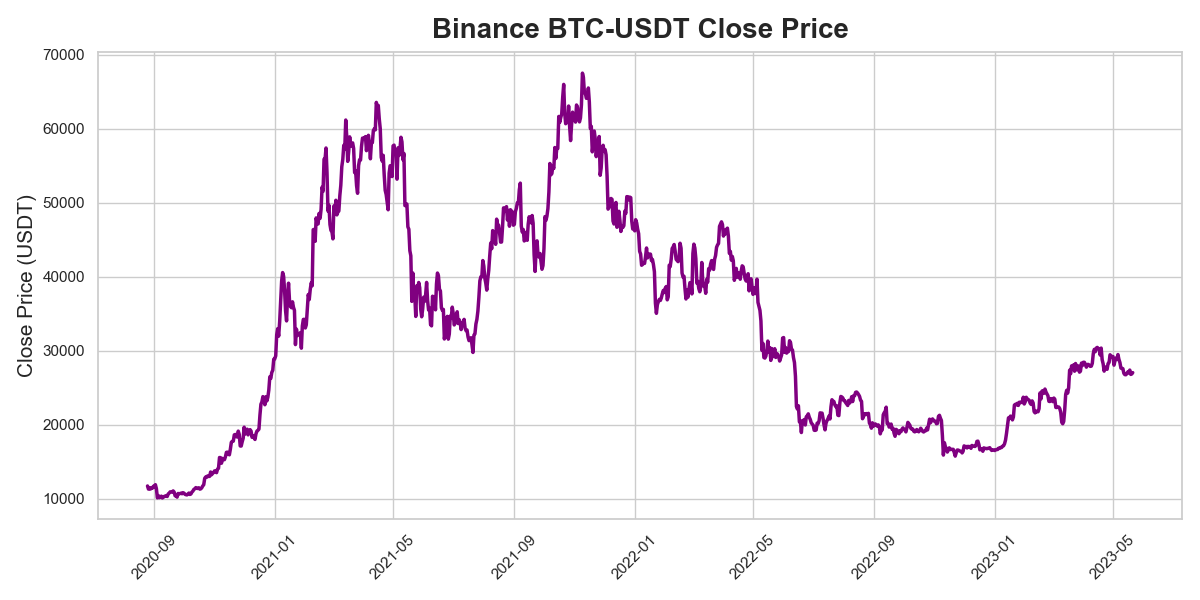
\includegraphics[width=1.0\textwidth]{Figs/BTC-USD.png}
        \caption{BTC-USD daily close prices from 23rd August 2020 to 15th May 2023 obtained from Binance.~\citep{tradingview}}
        \label{fig:BTC-USD}
    \end{center}
\end{figure}

\begin{figure}[htbp]
    \begin{center}
        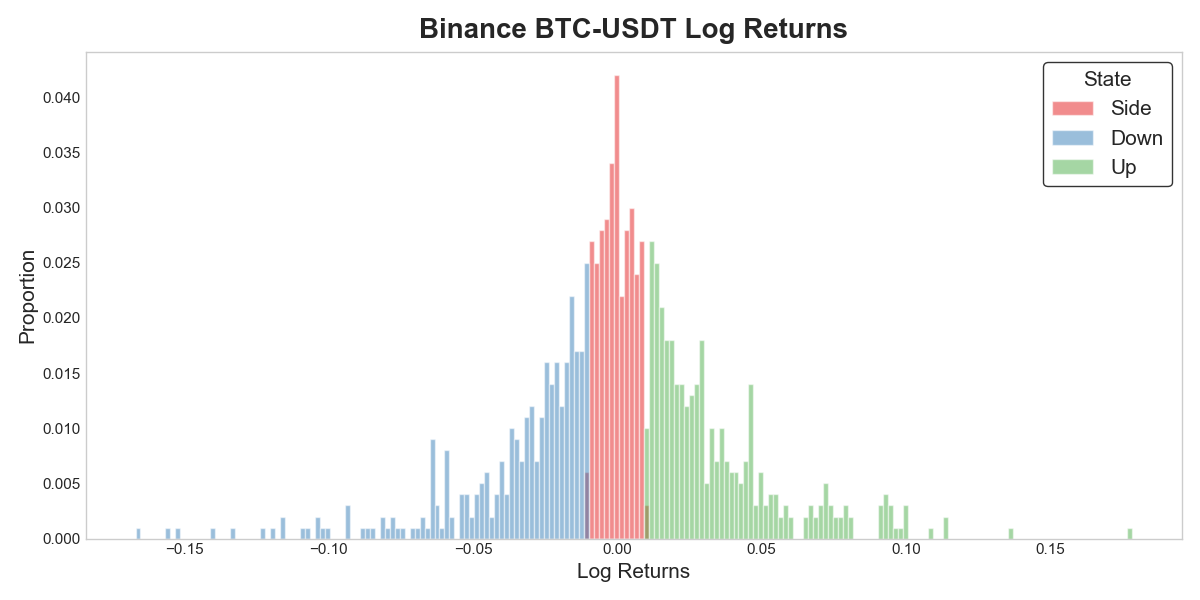
\includegraphics[width=1.0\textwidth]{Figs/BTC-USD_hist.png}
        \caption{Distribution of the log returns with respect to predefined market states.~\citep{tradingview}}
        \label{fig:BTC-USD-distribution}
    \end{center}
\end{figure}

Observing the distribution of the log-returns of the daily BTC-USDT close price in~\ref{fig:BTC-USD-distribution} we may conclude that such a random variable is normally distributed,
given the symmetric property of the distribution with respect to the mean value. Furthermore, it is visible that the kurtosis might be greater than 3,
which implies that the distribution has heavier tails than the normal distribution, i.e.\ the extreme events are more likely to occur than in the normal distribution.
Such a property is also called \textit{leptokurtic} distribution which is a result of the high volatility of the cryptocurrency market.~\citep{Peters1994}

Let us now take the ordered sample of states from the BTC-USDT close price time series data and calculate 
the transition and initial probabilities for each state as follows:

\begin{equation}
    \textbf{A} = \begin{pmatrix}
     0.22 & 0.16 & 0.62 \\
     0.32 & 0.27 & 0.41 \\
     0.6 & 0.19 & 0.21 \\
     \end{pmatrix}
     , \quad 
     \textbf{p} = \begin{pmatrix}
     0.4 & 0.19 & 0.41 \\
     \end{pmatrix}
 \end{equation}

where we note that the frequency of observing each state is proportional to the initial distribution $\textbf{p}$, and we assume that state space is $I = \{U,S,D\}$ 
By the definition of the transition matrix $\textbf{A}$, such matrix is also a stochastic matrix since it satisfies the properties given by Equation (1.5).
Each state of the transition matrix $\textbf{A}$ is also non-absorbing since the probability of observing a state $i$ at time $t+1$ given the state $j$ at time $t$ is greater than 0 
and aperiodic since the greatest common divisor of the lengths of all cycles in the chain is 1. Positive recurrence of each state is satisfied as well.
Furthermore, we may also conclude that the state space is irreducible since all states communicate with each other, i.e.\ there is a non-zero probability of transitioning from any state to any other state.
Therefore, we may conclude that the Markov Chain is ergodic, and the stationary distribution exists, is unique and is approximated by the initial distribution $\textbf{p}$ using Equation~\ref{eq:stationary}.
Finally, we may also calculate the expected return time for each state as follows:

\begin{align}
    E[\tau_U(1)|X_0=U] &= \frac{1}{\pi_U} = \frac{1}{0.4} = 2.5 \\
    E[\tau_S(1)|X_0=S] &= \frac{1}{\pi_S} = \frac{1}{0.19} = 5.26 \\
    E[\tau_D(1)|X_0=D] &= \frac{1}{\pi_D} = \frac{1}{0.41} = 2.5
\end{align}

where $\pi$ is the stationary distribution of the Markov Chain. In other words, the expected time of returning to 
state $U$ and $D$ is 2.5 days, and 5.26 days for state $S$. Although, the expected return times provide interesting behavioral insights,
they are simplified by the Markov property of memoryless process, stock and cryptocurrency markets do have certain memory and path-dependence properties as well as they 
are effected by external factors such as news, social media, etc. Therefore, the expected return times are only approximations of the real expected return times.

\section{Continous-time Markov Chains}~\label{sec:ctmc}

In the previous section we have considered a discrete-time Markov Chains, i.e.\ the state space and transition period was discrete. Such period means that 
the chain can stay in a state for integer number of time steps before transitioning to another state. 
For continous-time Markov Chains we will assume that the transition period is continuous, more specifically, the period is exponentially distributed with parameter $\lambda$.

Let us consider a stochastic process $\{X(t),t \geq 0\}$ on a probability space $(\Omega,\mathcal{F},\mathbb{P})$ s.t.\ for all $t \in \mathbb{R}_0^+$ and $i_0,i_1,\ldots,i_{t+1} \in I$ it holds that:

\begin{equation}
\mathbb{P}(X(t)=j|X(s)=i, X(t_n)=i_n,\ldots,X(t_1)=i_1) = \mathbb{P}(X(t)=j|X(s)=i)
\end{equation}

where $0 \leq t_1 < \cdots < t_n < s < t $ and so it is trivially seen that such expression is equivalent to the discrete-time Markov Chain property 
given by Equation~\ref{eq:DTMC} with the only difference of continuous transition period.~\citep{Tolver2016}

Since the state space remains the same as in discrete-time Markov Chains, we refer to the same transition matrix $\textbf{A}$ and initial distribution $\textbf{p}$.
In upcoming subsection, continuous-time Markov Chain is assumed to be homogeneous, i.e.\ the transition probabilities are independent of time:

\begin{equation}
p_{i,j}(s,s+t) = p_{i,j}(t), \quad i,j \in I
\end{equation}

which also implies that the transition probability is determined only by the length of the transition period $t$. 
Chapmam-Kolmogorov equality for $s,t \geq 0$ also holds for continous-time Markov Chains:

\begin{equation}
p_{i,j}(s+t) = \sum\limits_{k \in I} p_{i,k}(s) p_{k,j}(t), \quad i,j \in I
\end{equation}

Here we also assume \citep{Gallager2013} stating following:

\begin{equation}
    \lim_{t \to 0_{+}} p_{i,j}(t) = \delta_{i,j} = 
        \begin{cases}
            1, & \text{if } i = j\\
            0, & \text{if } i \neq j
        \end{cases}
\end{equation}

where $\delta_{i,j}$ is a \textit{Kronecker delta function}, i.e.\ the transition probabilities $p_{ij}(t)$ are right continuous at $t=0$.~\citep{Norris2012} says that if such additional conditions are satisfied for any homogeneous continous-time Markov Chain, 
then the underlying stochastic process is said to be continuous and there exists its version that is separable, measurable and its trajectories are càdlàg almost surely. Such version allows us to infer 
certain properties of the stochastic process.

For example \citep{Gidi2018}, one important property of such Markov Chain following from \textit{Doob's martingale convergence theorem} for $s \geq 0$ and $h>0$ is:

\begin{equation}
    \mathbb{P}(X(t) = i|X(s)=i, s \leq t \leq s+h) = \exp(-{q_i}h)
\end{equation}

which means that the probability of staying in state $i$ for time $h$ is equal to $e^{-{q_i}h}$. 
Non-negative real elements of $q_{i,j}$ are called \textit{transition rates} from state $i$ to state $j$ and absolute transition 
rate $q_i = \sum_{j \neq i} q_{i,j}$ respectively. Let us denote $\textbf{Q}$ as transition rates matrix with entries $\{q_{i,j}: i,j \in I\}$ where each row sums to zero, i.e. $\sum_{j \in I} q_{i,j} = 0$. 
This also means that the diagonal entries of $\textbf{Q}$ are equal to $q_i = -q_{i,i}$ and $\sum_{j \neq i} q_{i,j} = -q_{i,i}$. 
Trivially, in cases where the transition rate $q_i=0$, the $p_{i,i} = 1$, i.e.\ the state $i$ is absorbing, 
once the chain enters such state it remains in such state for infinite amount of time. On the contrary, if $0 < q_i < \infty$ then the state $i$ is non-absorbing and stable, therefore
the chain will eventually leave such a state. For infinite transition rate $q_i = \infty$ the state $i$ is called \textit{unstable} where the time of staying in such state is almost surely zero.~\citep{Praskova2012}

If we consider a stable state $i$ then its expected time of staying in such state is exponentially 
distributed with expected value of $1/q_i$. In other words, the expected time of staying in state $i$ is equal 
to the inverse of the transition rate $q_i$.~\citep{Norris2012}

Since, we have already defined that the process has exponentially distributed transition period, we may define a \textit{holding time} $T_i$ as a random variable that denotes the time of staying in state $i$:

\begin{equation}
T_i = \inf \{t \geq 0 : X(t) \neq i | X(0) = i\}
\end{equation}

from which it follows that $\mathbb{P}(T_i>s) = P(X_t=i,0 \leq t \leq s|X_0=i) = e^{-q_i s}$ and its probability density functions is:

\begin{equation}
    f(x) = 
    \begin{cases}
        q_i e^{-q_i x}, & x \geq 0\\
        0, & \text{elsewhere}
    \end{cases}
\end{equation}

According to \citep{Praskova2012} and the properties of the transition rates, such time-homogeneous continuous Markov Chain should satisfy following equations:

\begin{equation}
    \begin{aligned}
        \mathbb{P}(X_{t+h}=i|X_t=i) &= 1 - q_i h + o(h) \\
        \mathbb{P}(X_{t+h}=j|X_t=i) &= q_{i,j} h + o(h), \quad i \neq j
    \end{aligned}
\end{equation}

where $o(h)$ is a function of $h$ such that $\lim_{h \to 0} \frac{o(h)}{h} = 0$.

Such intensities resemble the probability functions of Poisson process, and indeed according to \citep{Norris2012} it is a special case of homogeneous continous-time Markov Chain with intensity $\lambda \geq 0$ if following conditions are satisfied:

\begin{itemize}
\item [1)] Stochastic process is viewed as a jump process, i.e.\ current state $i$ either stays in state $i$ or jumps to another state $j=i+1$. Therefore, given an interval $[t,t+h]$ the probability of jumping to another state is $\lambda h + o(h)$ and the probability of staying in state $i$ is $1-\lambda h + o(h)$.
\item [2)] Intensity $\lambda$ is constant, i.e.\ the probability of jumping to another state is independent of time, i.e. depends only on the length of the interval. We refer to such process as homogeneous Poisson process.
\item [3)] Number of jumps in disjoint intervals are independent, i.e.\ the probability of jumping to another state in disjoint intervals $[t_1,t_1+h]$ and $[t_2,t_2+h]$ is equal to the probability of jumping to another state in interval $[t_1,t_1+h] \cup [t_2,t_2+h]$.
\item [4)] The probability of more than one jump in a sufficiently small interval is negligible, i.e. the probability of jumping to another state in interval $[t,t+h]$ is $o(h)$.
\item [5)] Process starts in state $i=0$ at time $t=0$.
\end{itemize}

In a case of constant return rates, the matrix $\textbf{Q}$ with entries $q_{i} = - \lambda$ and $q_{i,j} = \lambda$ as follows:

\begin{equation}
    \textbf{Q} = 
    \begin{pmatrix}
    -\lambda & \lambda & 0 & 0 & \ldots \\
    0 & -\lambda & \lambda & 0 & \ldots \\
    0 & 0 & -\lambda & \lambda & \ldots \\
    \vdots & \vdots & \vdots & \vdots & \ddots \\
    \end{pmatrix}
\end{equation}

\subsection{Cryptocurrency market movements II.}


\section{Markov Renewal process}

Poisson process as a counting process serves as model to represent the number of events occurring in a given time interval $[0,t]$. The inter-arrival times 
between events are exponentially distributed iid random variables with parameter $\lambda>0$ and the number of events in all disjoint intervals is independent.
In other words, the probability of observing $n$ events in interval $[0,t]$ is given by Poisson distribution with parameter $\lambda t$. But we would like to also
study instances where the inter-arrival times are not exponentially distributed, but rather follow some other distribution.

Therefore, we introduce a concept of \textit{renewal process}, as stated by \citep{Praskova2012} and \citep{Mitov2014}, which can be defined using a sequence of non-negative random variables $\{X_n,n \in \mathbb{N}_0\}$ that are identically distributed and independent with 
distribution function $F(0)<1$ that satisfies following equation:

\begin{equation}
    T_n = \sum_{k=0}^{n} X_k, \quad n \in \mathbb{N}_0
\end{equation}

where $T_n$ is a random variable that denotes the occurence time of $n+1$-th renewal such that the renewal process $\{N_t,t \geq 0\}$ is then:

\begin{equation}
    N_t = \sup\{n: T_n \leq t\} = \sum_{n=1}^{\infty} \mathbbm{1}_{\{T_n \leq t\}}
\end{equation}

where $N_t$ is a random variable that denotes the number of renewals in the interval $[0,t]$. Furthermore, we could also note that the renewal function is 
derived as the expectation $m(t)=\mathbb{E}[N_t]$.

Our interest lies in the special case of the renewal process called \textit{Markov renewal process} which is defined as a renewal process with the additional property 
that the sequence of random variables $\{X_n,n \in \mathbb{N}_0\}$ denoting states still constitutes a Markov Chain, in this case discrete-time Markov Chain, and the transition intervals $\tau_n = T_n - T_{n-1}$ follow
any distribution with finite mean and its parameter may depend on the previous state $X_{n-1}$ and also current state $X_n$ of the Markov Chain. This process is also known as
\textit{semi-Markov} since the transitions between states are still occurring according the Markov Chain, but the time between transitions is a random variable with some distribution that again
may depend on the previous and current state of such Markov Chain. Thus, semi-Markov process serves as a way of describing the underlying Markov renewal process.~\citep{Medhi2012}

Take a process $\{X_n,n \in \mathbb{N}_0\}$ defined on state space $I$ and let the transitions occur at certain epochs $t_0=0,\dots,t_n,t_{n+1}$. If for such process Markov memoryless property holds:

\begin{equation}
    \mathbb{P}(X_{n+1}=j, \tau_{n+1} \leq t|X_n=i,\ldots,X_0=i_0,t_n,\ldots,t_0) = \mathbb{P}(X_{n+1}=j, \tau_{n+1} \leq t|X_n=i)
\end{equation}

then the $\{X_n,\tau_n\}$ for $n \in \mathbb{N}_0$ constitute a \textit{Markov renewal process}, as stated by \citep{Cinlar1969} and \citep{Barbu2008}, and the process is clearly time-homogeneous since the transition probabilities are independent of time:

\begin{equation}
    \mathbb{P}(X_{n+1}=j, \tau_{n+1} \leq t|X_n=i) = \textbf{Q}_{i,j}(t)
\end{equation}

where $\textbf{Q}_{i,j}(t)$ is, according to \citep{Medhi2012}, called a \textit{semi-Markov kernel} of the Markov renewal process. Limiting behavior of the kernel $\textbf{Q}_{i,j}(t)$ as $t \to \infty$ 
is approaching the transition matrix $\textbf{A}$ of the Markov Chain since the distribution function of waiting times is equal to 1 for $t \to \infty$:

\begin{equation}
    \lim_{t \to \infty} \textbf{Q}_{i,j}(t) = a_{i,j}
\end{equation}

Moreover, for continuous process $\{Y(t)\}$ defined on a state space $I$, we say that it is called \textit{semi-Markov process} if:

\begin{equation}
    Y(t) = X_n, \quad t \in [t_n,t_{n+1})
\end{equation}

where $X_n$ is an embedded Markov Chain of such continuous process. Clearly, we see that at each epoch $t_n$ the process $\{Y(t)\}$ jumps to a new state and stays in such state until the next epoch $t_{n+1}$ as is visible on Figure~\ref{fig:semi_markov}. 
Therefore, the process $\{Y(t)\}$ is a semi-Markov process with semi-Markov kernel $\textbf{Q}_{i,j}(t)$. From the definition of the continuous-time Markov Chain, it follows that the 
semi-Markov process with exponential holding times is a continuous-time Markov Chain \citep{Sahner1996}:

\begin{align}
    \mathbb{P}(X_{n+1}=j, \tau_{n+1} \leq t|X_n=i) &= \mathbb{P}(X_{n+1}=j|X_n=i) \mathbb{P}(\tau_{n+1} \leq t|X_{n+1}=j, X_n=i) \\ 
                                                   &= \mathbb{P}(X_{n+1}=j|X_n=i) \textbf{W}_{i,j}(t) \\
                            \textbf{Q}_{i,j}(t)    &= a_{i,j} (1-e^{- \lambda_i t})
\end{align}

where $\textbf{W}_{i,j}(t)$ is a probability that the process $\{Y(t)\}$ stays in state $j$ for time $t$ given that it is in state $i$, i.e. waiting time. In other words, it is a conditional distribution function 
of the random variable $\tau$ conditioned on the events $X_{n+1}=j, X_n=i$. Such cumulative distribution function is again a random variable we call \textit{conditional sojourn time} and denote with $T_{i,j}$:

\begin{equation}
    \textbf{W}_{i,j}(t) = \mathbb{P}(T_{i,j} \leq t) = \mathbb{P}(\tau_{n+1} \leq t|X_{n+1}=j, X_n=i) 
\end{equation}

we can also find the relation between waiting times and transition probabilities as follows from Equation~\ref{eq:semi_markov} which holds for all $a_{i,j} > 0$ s.t.\ if transition probability to state $j$ is zero, 
i.e. $a_{i,j} = 0$, then the waiting time is assumed to be 1:

\begin{equation} \label{eq:semi_markov}
    \textbf{W}_{i,j}(t) = \frac{\textbf{Q}_{i,j}(t)}{a_{i,j}}
\end{equation}

\begin{figure}[htbp]
    \begin{center}
        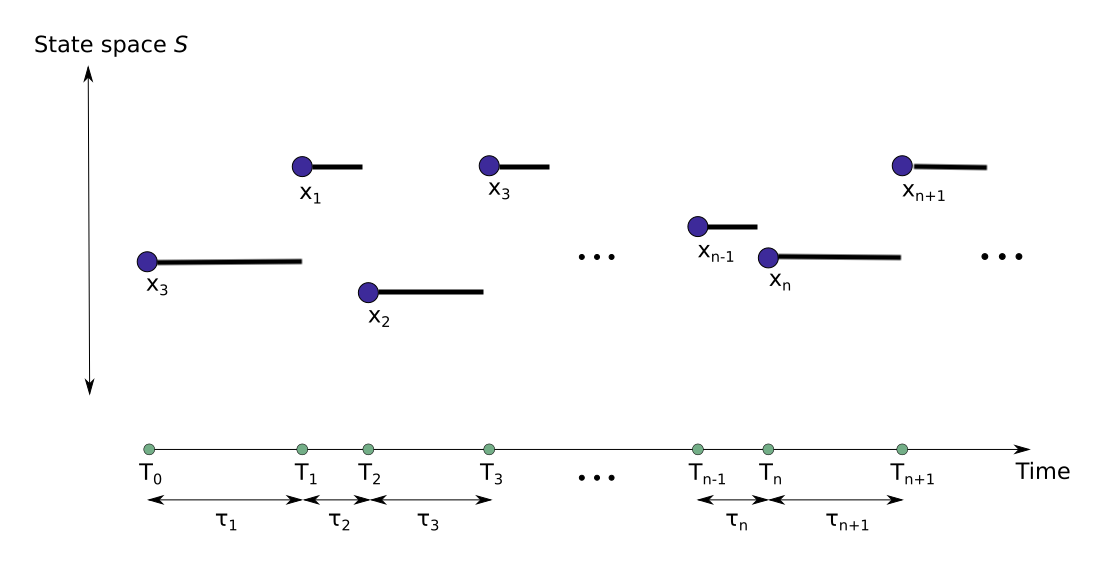
\includegraphics[width=1.0\textwidth]{Figs/semi_markov.png}
        \caption*{\textbf{Source:} \href{https://en.wikipedia.org/wiki/Markov_renewal_process}{\textit{Wikipedia page on Markov renewal process}}}
        \caption[Diagram representation semi-Markov process]{Graphical representation of a semi-Markov process Y(t).}
        \label{fig:semi_markov}
    \end{center}
\end{figure}

Thus, we can observe that the there is a valuable benefit of using more generalized Markov Chain such as semi-Markov process since it allows us to model the waiting times between transitions
as a random variable with some distribution. In other words, we can model the time between transitions as a random variable with some distribution, which is not possible with the standard (discrete-time) Markov Chain that
assumes that transitions occur at each time step and the time spent in each state (or inter-arrival time) is geometrically, or in continuous case exponentially, distributed. Subsequently in Section~\ref{sec:hsmm}, we shall introduce the Hidden semi-Markov Model (HSMM) 
where the semi-Markov process is used to represent the hidden state process.

This property is especially useful in modeling the cryptocurrency market since the time between transitions is not constant, but rather follows some distribution. We can expect that 
if the market is in bull or bear state it will stay in such state for some time, but the time spent in such state could be very different from stagnant market state.
